\documentclass[acmsmall,nonacm]{acmart}
\makeatletter
\renewcommand\@formatdoi[1]{\ignorespaces}
\makeatother

\usepackage{subcaption}
\usepackage{float}
\usepackage{tabularx}
\usepackage{graphicx}
\usepackage{caption}


%%
%% \BibTeX command to typeset BibTeX logo in the docs
\AtBeginDocument{%
  \providecommand\BibTeX{{%
    \normalfont B\kern-0.5em{\scshape i\kern-0.25em b}\kern-0.8em\TeX}}}


\begin{document}

\begin{titlepage}
  \begin{center}
      \vspace*{1cm}
      
      \huge\textbf{Natural Language Inference on a small Multilingual Dataset}

      \vspace{0.5cm}
           
      \vspace{1.5cm}
      \large
      \textbf{Lukas Timpl (lukti619)} \\
      \textbf{TDDE16} \\
      \vspace{0.8cm}
      Code: \href{https://github.com/lukas-jkl/nli-text-mining-project}{github.com/lukas-jkl/nli-text-mining-project}

      \vfill
             
      \vspace{0.8cm}
       
      Department of Science and Engineering\\
      Link\"{o}ping University\\
           
  \end{center}
\end{titlepage}

%%
%% The "title" command has an optional parameter,
%% allowing the author to define a "short title" to be used in page headers.
\title{Natural language inference on a small multilingual dataset}

%%
%% The "author" command and its associated commands are used to define
%% the authors and their affiliations.
%% Of note is the shared affiliation of the first two authors, and the
%% "authornote" and "authornotemark" commands
%% used to denote shared contribution to the research.
\author{Lukas Timpl}
\email{lukti619@student.liu.se}


%%
%% The abstract is a short summary of the work to be presented in the
%% article.
\begin{abstract}
The goal of this project was to explore different methods of natural language processing and investigate how they compare on a small and challenging dataset in the task of natural language inference (NLI). We investigate different methods and see how they perform in this scenario. 
We explore simpler methods of neural networks trained with manual features as well as word embeddings, recurrent neural networks and finally transformer architectures. 
We also explore the topic of pretraining in this context since the used dataset is relatively small. Another challenging aspect of the dataset is that it does not only contain English samples but samples from 15 different languages. We tackle this problem both by using translation as well as multi-lingual models and compare both approaches.
\end{abstract}

%%
%% The code below is generated by the tool at http://dl.acm.org/ccs.cfm.
%% Please copy and paste the code instead of the example below.
%%
\begin{CCSXML}
<ccs2012>
   <concept>
       <concept_id>10010147.10010178.10010179</concept_id>
       <concept_desc>Computing methodologies~Natural language processing</concept_desc>
       <concept_significance>500</concept_significance>
       </concept>
 </ccs2012>
\end{CCSXML}

%\ccsdesc[500]{Computing methodologies~Natural language processing}
%%
%% Keywords. The author(s) should pick words that accurately describe
%% the work being presented. Separate the keywords with commas.


%%
%% This command processes the author and affiliation and title
%% information and builds the first part of the formatted document.
\maketitle

\tableofcontents


\section{Introduction}
% Introduce the task or research question that you have addressed in
% your project. What were you trying to do? Why did you choose this project?
When companies are faced with a task in natural language processing, in many cases, there is no big dataset for training available. Another big problem is languages. 
While the majority of users might be from a particular country speaking the same language, additionally, there might be smaller groups of users in various different countries speaking vastly different languages.
This makes natural language processing even more challenging.
In this project, we explore these problems by using a small dataset consisting of 15 different languages and the task of natural language inference (NLI). To address the problem of our small dataset, we try different strategies of using pretrained word embeddings, pretraining our models on other datasets, and using already pretrained models. We also explore different methods for dealing with a large set of languages. In this context, we utilize translation as well as multi-lingual models. Instead of just aiming for the best performing model, we also compare models by their size as training and inference on large models can increase costs significantly.  

\section{Theory}
% Relevant theoretical background and models used
In this section we discuss the theoretical background and models that where used in this project.

\subsection{Natural Language Inference (NLI)} \label{sec:nli}
Natural language inference is a central task in natural language processing, and the concepts of entailment and contradiction are eminent in understanding languages~\cite{snli-bowman2015}. Hence, this topic also plays an important role in tasks such as information retrieval and common-sense reasoning~\cite{snli-bowman2015}. In the three label NLI classification task, the model is given two sentences: a premise and a hypothesis. The goal is to detect whether the premise entails or contradicts the hypothesis or whether both sentences are neutral to each other. Therefore there exist three different labels: entailment, contradiction, and neutral. 


\subsection{Neural Networks}
Neural networks have provided outstanding performance in many classification tasks. %TODO ref
So naturally they where and are frequently used in natural language processing. A challenging aspect with text as input is the transformation into numerical features that can be processed by the network. 

\subsubsection{Unigram Feature}
A simple method, which also requires little processing, is to encode each word in the vocabulary as a single number. We refer to a sentence encoded into these numbers as its unigram features.

\subsection{Word Embeddings}
Another option for encoding words is to encode each word as a vector. Each word from the vocabulary is mapped to a d-dimensional vector. Word embeddings can be used as a form of transfer learning. We can use existing embedding vectors pretrained on a large corpus and use them to encode the words for our specific task. This has been done successfully for a variety of applications in natural language processing such as information retrieval or document classification~\cite{glove-pennington2014}.

\subsubsection{GloVe - Global Global Vectors for Word Representation}
In this project, we utilize the GloVe word embeddings~\cite{glove-pennington2014}. GloVe is an unsupervised learning method for generating vector representations of words. The learning algorithm uses co-occurrences of words in a corpus, that is, how often a word occurs in the context of another word~\cite{glove-pennington2014}. A word is said to be in the context of another word if it appears within a context window around it. The algorithm also weights this co-occurrence stronger depending on the distance between the words~\cite{glove-pennington2014}.

\subsection{Recurrent Neural Networks (RNNs)}
Instead of using standard feed-forward neural networks, another approach is to utilize recurrent neural networks. This type of network is capable of modeling sequential data~\cite{rnn-salehinejad2018recent}. Hidden states in the network work as a form of memory, where a new state is conditioned on the previous state of the network. This allows RNNs to remember previous inputs over a time period~\cite{rnn-salehinejad2018recent}. 

\subsubsection{Long-Short Term Memory (LSTM)}
Problems with the standard design of recurrent neural networks are exploding and vanishing gradients~\cite{rnn-salehinejad2018recent}. Long-Short Term Memory networks~\cite{lstm-hochreiter1997long} are an architecture frequently used to tackle these problems. In this architecture, there are gates that control the hidden units. There are input and output gates that control the flow of information as well as forget gates that scale when the input of the memory cell should decay~\cite{rnn-salehinejad2018recent}.

\subsection{Transformers}
One problem with LSTM networks is that they are very slow to train~\cite{rnn-salehinejad2018recent} and do not lend themselves well to parallel computation~\cite{attention-vaswani2017}, which prevents efficient training on GPUs. An architecture that also allows for processing sequences but does not suffer from these problems is the Transformer architecture~\cite{attention-vaswani2017} depicted in Figure~\ref{fig:transformer}. The architecture is split into two parts an Encoder and a Decoder.

\begin{figure}[h]
  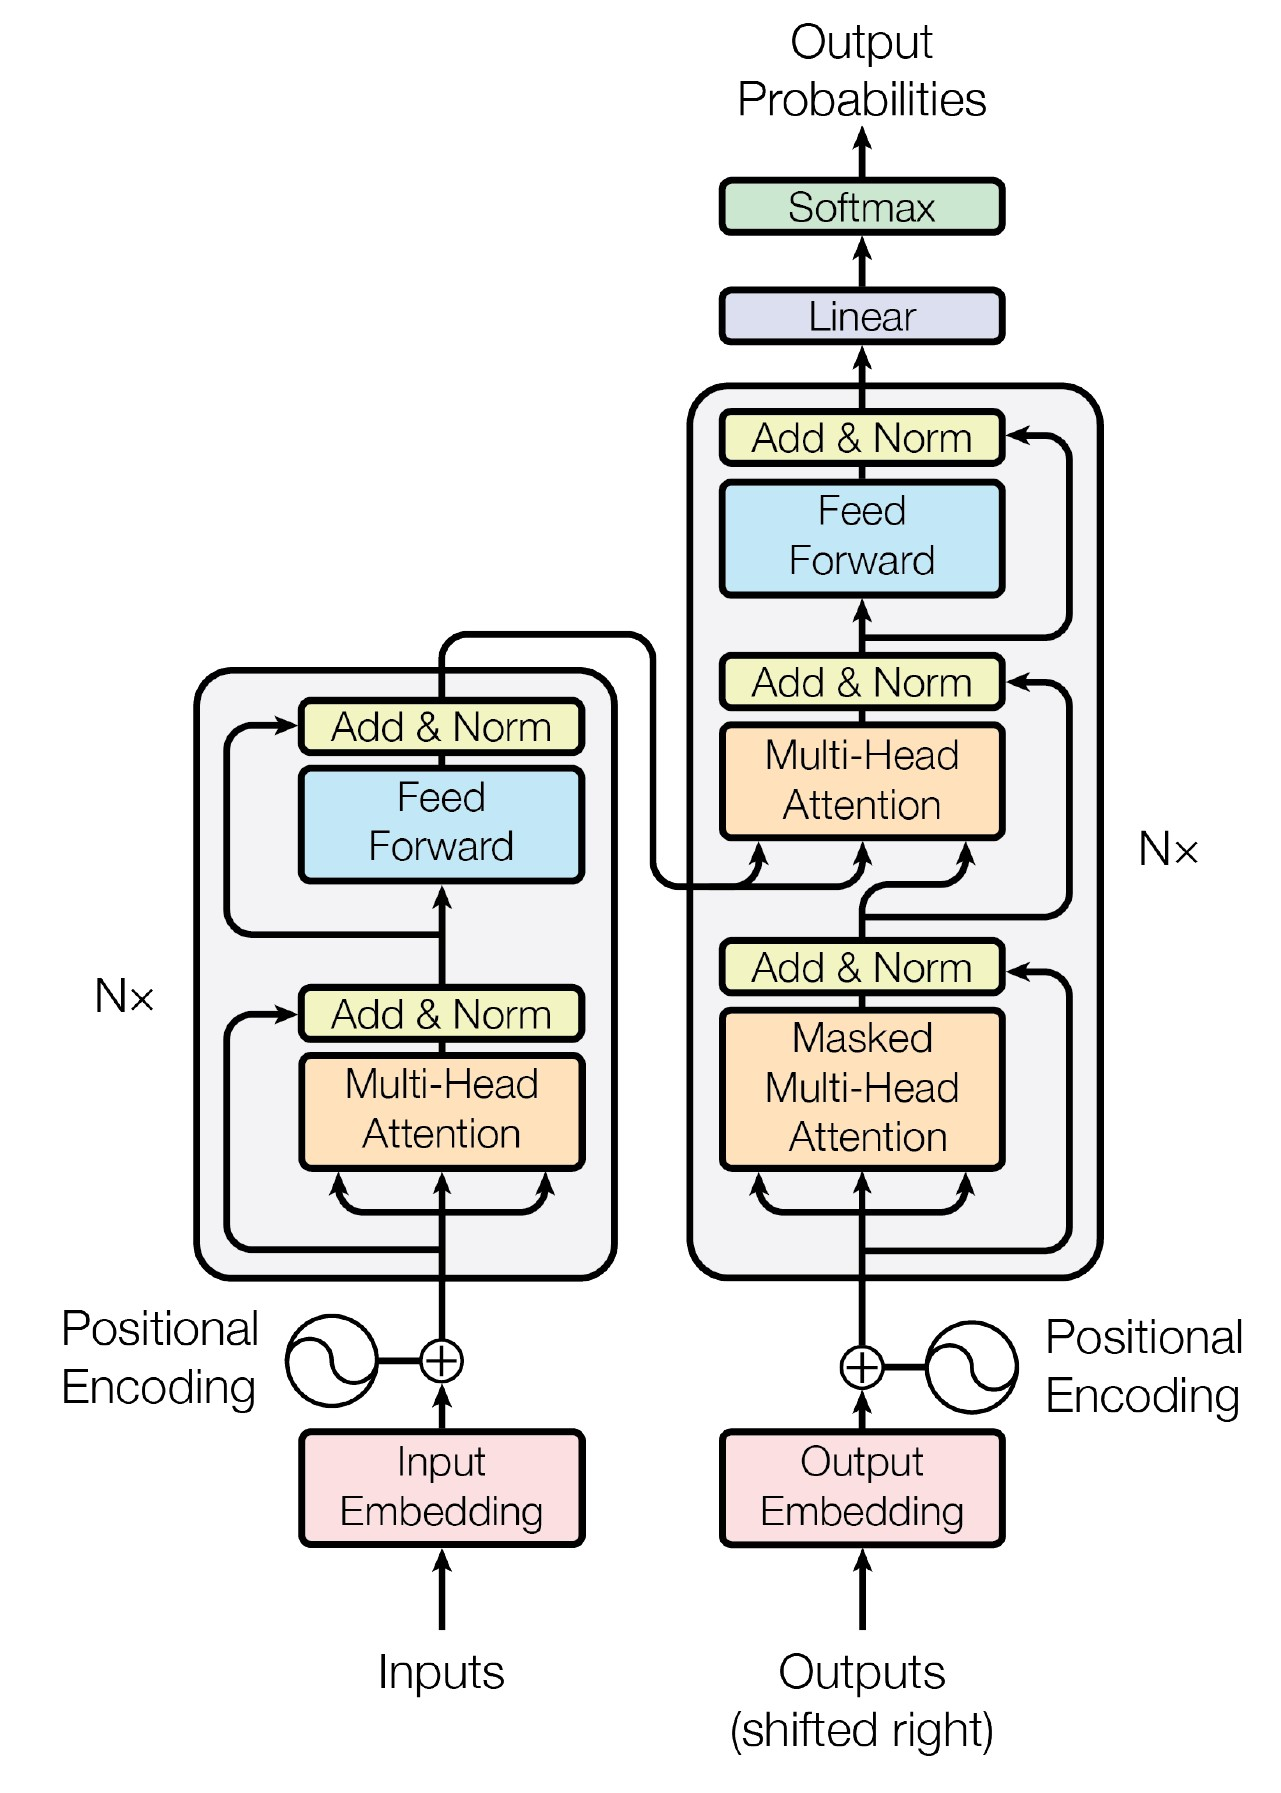
\includegraphics[width=0.3\textwidth]{assets/transformer_architecture.jpg}
  \caption{The transformer architecture, image taken from~\cite{attention-vaswani2017}.}
  \label{fig:transformer}
\end{figure}


\subsubsection{Encoder}
The encoder part, depicted on the left side in Figure~\ref{fig:transformer}, 
takes the input words and encodes them using standard word embeddings.
Additionally, the transformer has a positional encoder that produces vectors which not only depend on the words themselves, but also their position within the sentence~\cite{attention-vaswani2017}. These vectors are then processed by a multi-head attention and a feed-forward layer. The attention part essentially tells the transformer which parts of the sentence input are relevant together and produces attention vectors. These attention vectors are then processed in a conventional feed-forward network~\cite{attention-vaswani2017}.

\subsubsection{Decoder}
Transformers are typically trained in a sequence to sequence task. That is, they produce a sequence of outputs from a sequence of inputs, for example, a translation. The decoder, depicted on the right side of Figure~\ref{fig:transformer}, uses the part of the output sequence that is already produced by the transformer and again encodes it in positional encoding and performs the attention mechanism. This is then combined with the encoder output in another attention block which is then followed by a feed-forward layer~\cite{attention-vaswani2017}.

\subsubsection{BERT}
The transformer architecture was well received and inspired new architectures. The architecture BERT~\cite{bert-devlin2019} stands for Bidirectional Encoder Representation from Transformers. It takes the encoder idea from the transformer architecture and stacks multiple encoders together. While the Transformer architecture was specifically targeted at translation, BERT is a more general model that can be used at a variety of different tasks ranging from question answering to language inference~\cite{bert-devlin2019}.  
BERT is pretrained on two different tasks. Masked language modeling (Mask LM) in which it has to predict missing words in a sentence and next sentence prediction (NSP) where it has to determine given two sentences if one follows the other~\cite{bert-devlin2019}. The special token [CLS] is used at the beginning of the input and the token [SEP] for separating the two sentences. The training approach is depicted in Figure~\ref{fig:bert} after pretraining BERT can be fine-tuned for a variety of tasks such as question answering (SQuAD) or named entity recognition (NER)~\cite{bert-devlin2019}. 

\begin{figure}
  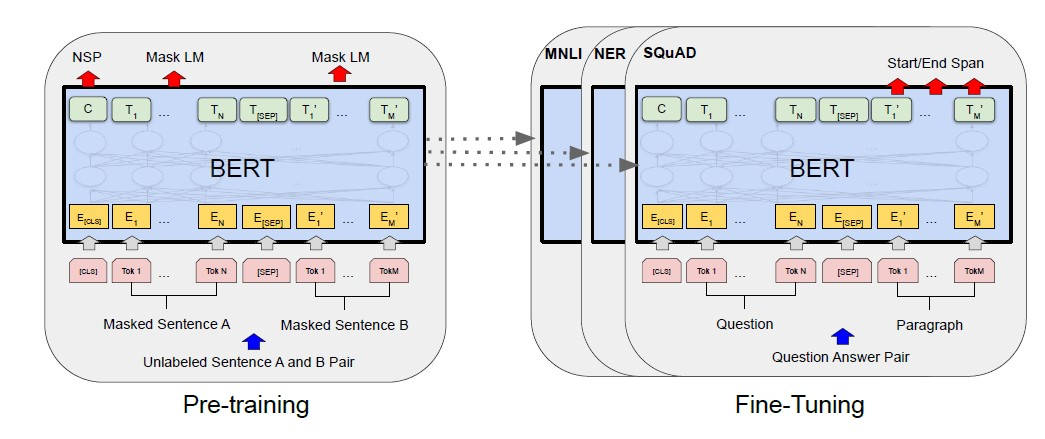
\includegraphics[width=0.8\textwidth]{assets/bert_architecture.jpg}
  \caption{Bert training procedure, figure taken from~\cite{bert-devlin2019}.}
  \label{fig:bert}
\end{figure}

\subsubsection{RoBERTa}
The RoBERTa model~\cite{roberta-liu2019}, which stands for robustly optimized BERT approach, builds on BERT and improves on the training and hyperparameter choices to create a model that performs even better than the original BERT.

\subsubsection{Multi-Lingual Models}
While the original BERT and RoBERTa models were only trained for English, new transformer models are available, which can process a variety of different languages~\cite{xlm-roberta-conneau2020unsupervised}.

\section{Data}
% present data, what information, where from, pre-processing
The dataset for this project was taken from Kaggle~\cite{kaggle-dataset}. 
It consists of 12,120 labeled and 5,195 unlabelled samples for the task of natural language inference with three labels as described in Section~\ref{sec:nli}. The labels 0, 1, and 2 are used for entailment, neutral, and contradiction respectably. 
A few samples from the dataset are listed in Table~\ref{tab:data_samples}.
For this project, we only used the labeled part of the dataset. Figure~\ref{fig:languages_lables} depicts the distribution of languages and labels for the data. We chose this dataset due to the variety of languages and the low number of samples making it a challenging dataset. There are samples from 15 different languages. The majority of which are in English, while there are only a few samples for each of the other languages. The number of samples is approximately the same for each label: 35\% for label 2 (contradiction), 33\% for label 0 (entailment), and 32\% for label 1 (neutral).
The length of the sentences in the number of tokens is depicted in Figure~\ref{fig:sentence_length}. While most sentences have a length below 50 tokens, several outliers have a length of over 200 tokens.

\begin{table}[]
  \resizebox{0.8\textwidth}{!}{%
  \begin{tabular}{p{45mm}|p{45mm}|l}
  \textbf{premise} & \textbf{hypothesis} & \textbf{label} \\ \hline
  or they had somebody at home that was ill that they had to tend to i mean you can't make it everybody & They did not have anything to do. & 2 (contradiction)  \\ \hline
  Daniel Yamins ist ein brillanter junger Mathematiker. & Herr Zamins ist gut in Mathe. & 0 (entailment) \\ \hline
  Si te alteras te vas a marear. & El calor excesivo puede causar mareos en algunos casos. & 0 (entailment) \\ \hline
  4 billion for mercury. & Cleaning up mercury pollution costs billions of dollars every year. & 1 (neutral)
  \end{tabular}
  }
  \caption{Examples taken from the labelled part of the dataset~\cite{kaggle-dataset} used for this project.}
  \label{tab:data_samples}
  \end{table}


\begin{figure}[!h]
  \begin{subfigure}[b]{0.48\textwidth}
    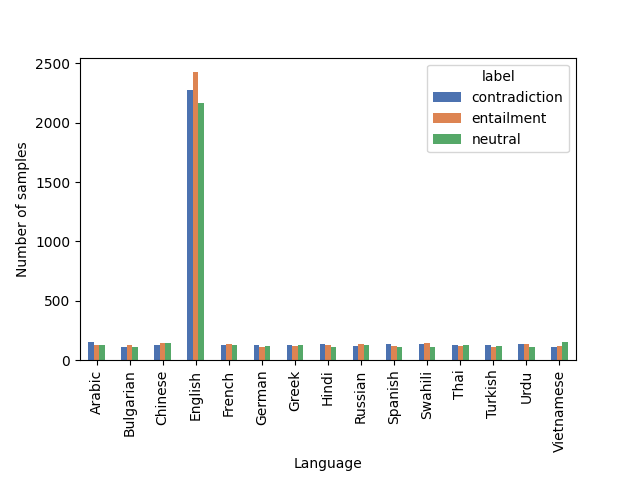
\includegraphics[width=\textwidth]{assets/label_hist.png}
    \caption{Distribution of samples across languages and labels.}
    \label{fig:languages_lables}
  \end{subfigure}
  \hfill
  \begin{subfigure}[b]{0.48\textwidth}
    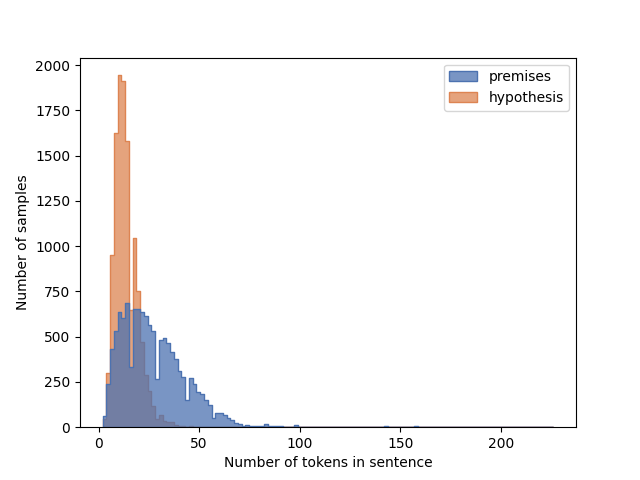
\includegraphics[width=\textwidth]{assets/length_hist.png}
    \caption{Distribution of sentence length in tokens across the dataset.}
    \label{fig:sentence_length}
  \end{subfigure}
  \caption{Distributions from the labeled part of the dataset~\cite{kaggle-dataset} used for this project.}
  \label{fig:dataset}
\end{figure}

\subsection{Pretraining Data}
In addition to the dataset from Kaggle~\cite{kaggle-dataset} we use the SNLI dataset~\cite{snli-bowman2015} with 570,000 samples as well as the MultiNLI~\cite{mlni-N18-1101} dataset with 433,000 samples for pretraining our models. Both contain samples for the same NLI task with three labels. However, all samples are in English.

\section{Method}
% explain how carried out, detailed enough to reproduce
For our experiments, we split the labeled part of the dataset into a train, and a test set 85\%/15\%. This gives us around 10,300 samples for training and around 1,800 for testing. We perform the experiments using scikit-learn and Tensorflow 2.
For all Tensorflow models, we used Adam as optimizer and sparse-categorical-cross-entropy as loss function. We use a validation set with a size of 20\% from the training data and early stopping to stop training if the validation loss does not decrease for several epochs.
If this does happen, we stop training and restore the weights to those that gave the lowest validation loss. The batch size for all our experiments is set to 32. 
We wanted to compare the performance of multilingual models with models using the same data translated to English. For this, we constructed a translated-English dataset which, additionally to the samples already available in English, contains data from other languages translated by Google Translate. 
To improve performance, we pretrain our models. However, we only use the full pretraining data for our final transformer models. All other models are pretrained with 100,000 samples from the SNLI dataset~\cite{snli-bowman2015}.

\subsection{Baseline}

\subsubsection{Guessing Baseline}
As baseline, we use random guessing based on the distribution of labels, which results in an accuracy of 35\%. 

\subsection{Feature-Based Models}

\subsubsection{Manual Feature Model}
The first model we train uses unigram features. We only count the occurrences of tokens in the sentences using scikit-learn's CountVectorizer. As classifier, we used a basic multilayer perceptron neural network with two layers of 64 and 32 neurons also created with scikit-learn. The activation function for the hidden layers is the ReLu function. The optimizer is Adam with default parameters from scikit-learn. 

\subsubsection{Word Embedding Model} %TODO: cite spacy?
For this model we used the \textit{en\_core\_web\_lg} model from spaCy, which uses GloVe common crawl vectors~\cite{glove-pennington2014} of size 300 to encode the input data. After encoding the words into vectors, we sum up all vectors for the premise and for the hypothesis, respectably. We then feed them into a neural network created using Tensorflow. The structure of the model is depicted in Figure~\ref{fig:embedding_model}. After the input, there are two layers for the hypothesis and two layers for the premise, each with 128 neurons. They are then concatenated and followed by two more layers with 512 neurons, followed by a final output layer of size three. All layers use the ReLu activation function, except for the final layer, which uses the Softmax function.  The learning rate for Adam is set to $1\times10^{-3}$.


\subsection{Sentence Vector Model (LSTM)} \label{sec:method_lstm}
The next model we train is an LSTM model. Again we create it using Tensorflow. 
For this model, we use embedding layers as part of the model. We initialize the embedding layers using the \textit{glove-twitter-100} vectors from Gensim and set them as not trainable to reduce the training time. The architecture is depicted in Figure~\ref{fig:lstm_model}.
We try various architectures with a different number of layers before and after the LSTM layer with a different number of neurons and also try dropout regularization in the LSTM layer. For these experiments, we utilize the keras-tuner with the Hyperband approach. Again all Dense layers use the ReLu activation except for the final layer, which uses Softmax. The LSTM uses a Tanh activation.  The learning rate for Adam is set to $1\times10^{-3}$.

\begin{figure}[h!]
  \begin{subfigure}[c]{0.35\textwidth}
    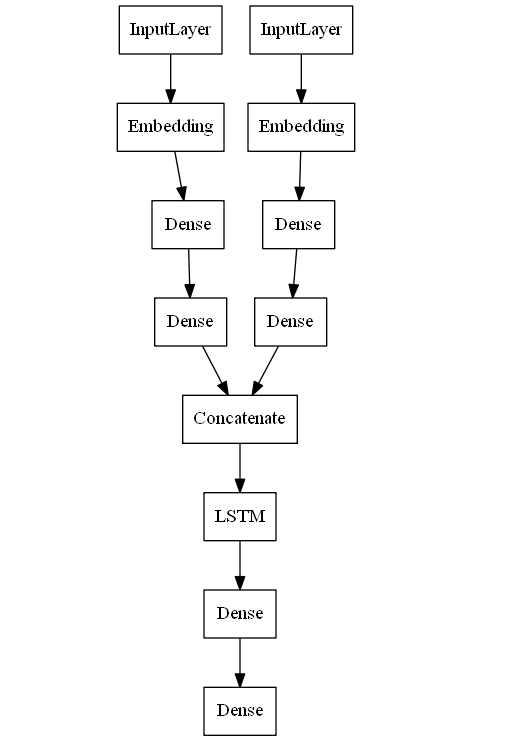
\includegraphics[width=\textwidth]{assets/lstm_model.png}
  \caption{Architecture for the sentence vector model (LSTM).}
  \label{fig:lstm_model}
  \end{subfigure}
  \hfill
  \begin{subfigure}[c]{0.35\textwidth}
    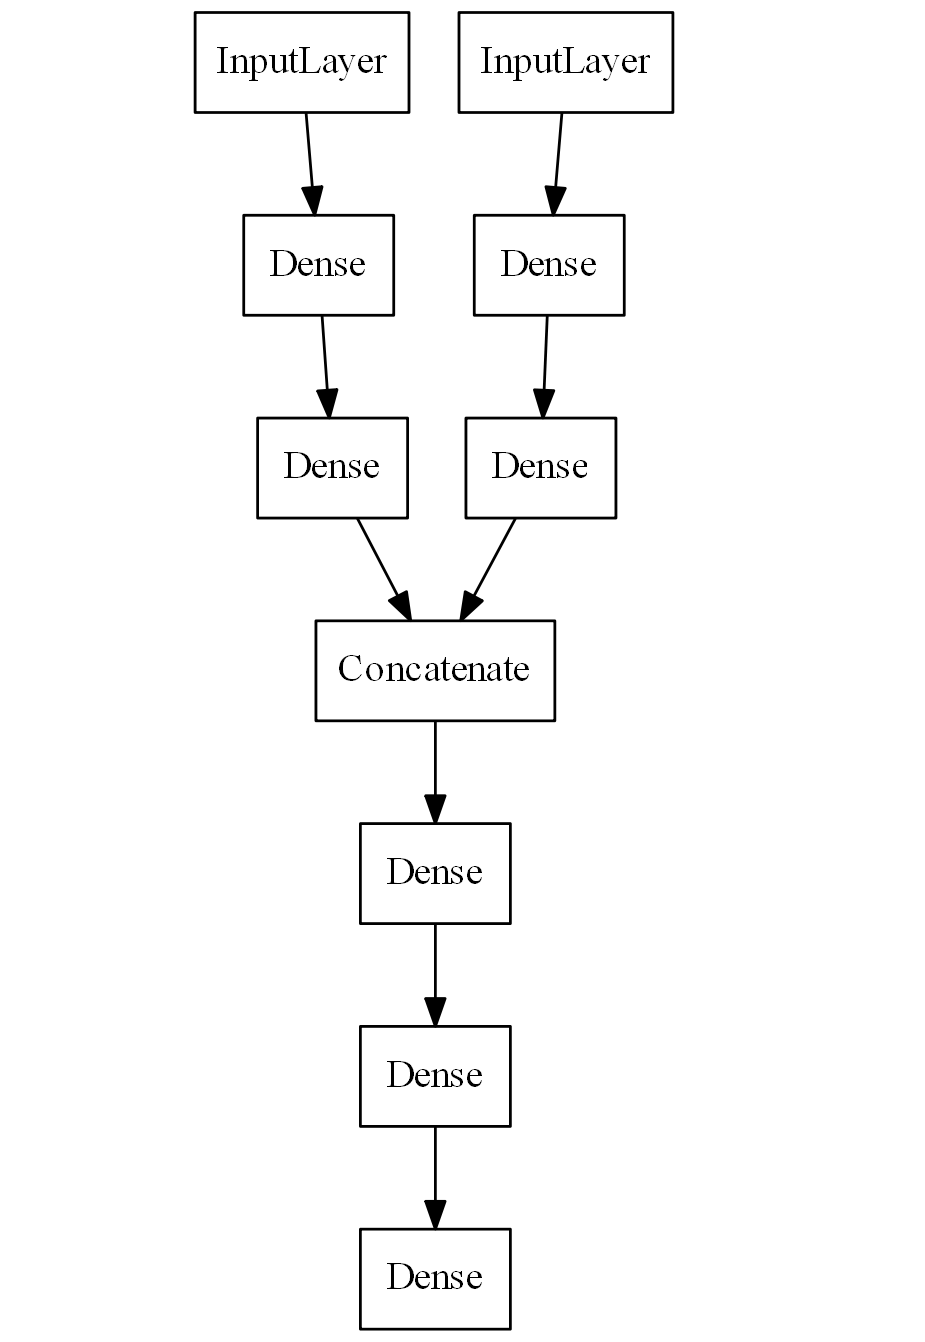
\includegraphics[width=\textwidth]{assets/embedded_model.png}
    \caption{Architecture of word embedding model.}
  \label{fig:embedding_model}
  \end{subfigure}
  \caption{Model architectures.}
  \label{fig:model_architectures}
\end{figure}




\subsection{Transformer Models} \label{sec:method_transformer}
The final type of models we train are pretrained transformer models in different sizes. We obtain the models from the transformers library~\cite{transformers-wolf-etal-2020} We limit the input size to 50 to reduce the hardware requirements for training. This still captures the majority of our data as can be seen in Figure~\ref{fig:sentence_length}. We use BERT and RoBERTa models by attaching additional layers. The two architectures are depicted in Figure~\ref{fig:transformer_models}. We build one architecture by only adding a single Dense layer with Softmax activation function and three outputs (Figure~\ref{fig:roberta_model}). Additionally, we create an architecture that uses a Pooling layer followed by a Dropout layer with dropout set to 0.1 and two Dense layers with ReLu activation of size 64 and 32 respectably. The final layer is again a Softmax and has size three.  The learning rate for Adam is set to $1\times10^{-5}$.

\begin{figure}[H]
  \begin{subfigure}[b]{0.35\textwidth}
    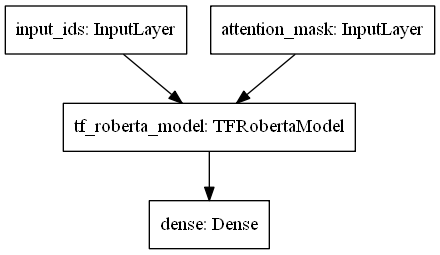
\includegraphics[width=\textwidth]{assets/roberta_model.png}
    \caption{Architecture used for transformer models, with only a final Dense layer attached.}
    \label{fig:roberta_model}
  \end{subfigure}
  \hfill
  \begin{subfigure}[b]{0.35\textwidth}
    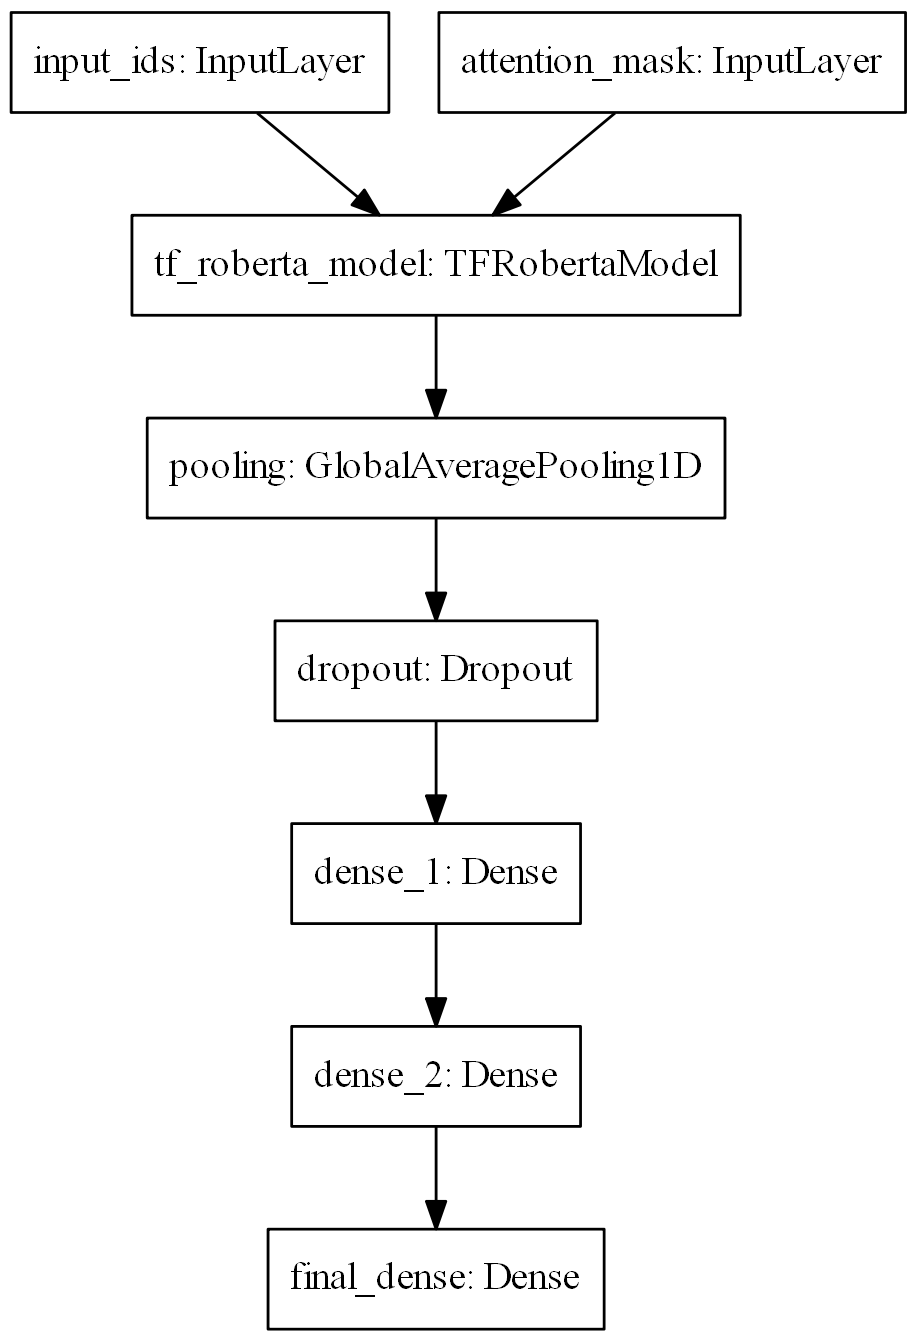
\includegraphics[width=\textwidth]{assets/roberta_model_maxpool.png}
    \caption{Architecture used for transformer models, with attached max-pool layer.}
    \label{fig:roberta_maxpool_model}
  \end{subfigure}
  \caption{Transformer models.}
  \label{fig:transformer_models}
\end{figure}



\section{Results}
% present results in objective way, use tables and charts and summary in text form. 
% Do not interpret your results.

\subsection{Feature-Based Models}

\subsubsection{Manual Feature Model}
As input, we only used unigram features from the hypothesis sentence. After four epochs of training, the model achieved a validation accuracy of 0.44 and a test accuracy of 0.46.
The results on the test set are depicted in Table~\ref{tab:manuel_feature_classification_report}. Figure~\ref{fig:manual_feature_confusion_matrix} shows the confusion matrix.

\vspace*{5ex}
\begin{minipage}[H]{\textwidth}
  \begin{minipage}[b]{0.49\textwidth}
    \centering
    %\rule{6.4cm}{3.6cm}
      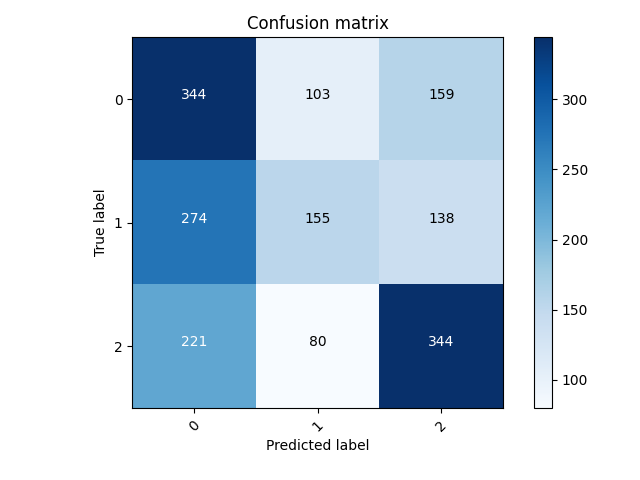
\includegraphics[width=0.8\textwidth]{assets/manual_feature_confusion_matrix.png}
      \captionof{figure}{Confusion matrix for the test set predictions of the feature-based model.}
      \label{fig:manual_feature_confusion_matrix}
  \end{minipage}
  \hfill
  \begin{minipage}[b]{0.49\textwidth}
    \centering
    \resizebox{0.9\textwidth}{!}{%
    \begin{tabular}[b]{|l|c|c|c|}
      \hline
      \multicolumn{1}{|c|}{label} &precision&recall&f1-score\\ \hline
      0 (entailment)&0.41&0.57&0.48\\
      1 (neutral)&0.46&0.27&0.34\\
      2 (contradiction)&0.54&0.53&0.53\\ \hline
      \multicolumn{3}{|c|}{accuracy} &\multicolumn{1}{c|}{0.46}\\
      \hline
      \end{tabular}}
      \newline
      \captionof{table}{Classification performance on the test set for the feature-based model.}
      \label{tab:manuel_feature_classification_report}
    \end{minipage}
  \end{minipage}

\subsubsection{Word Embedding Model}
We trained all word embedding models with a patience value of five. Therefore training is only stopped if the validation loss does not decrease for five epochs, but we show the full training graph. However, the weights are reset to the epoch, which reached the minimal validation loss marked in the graph.
For the word embedding model, we pretrained on 100,000 samples from the SNLI dataset~\cite{snli-bowman2015}. Figure~\ref{fig:embedding_model_pretrain} shows the accuracy on the training and validation set during pretraining. We also created a model without pretraining. The accuracy during training on the Kaggle dataset is depicted in Figure~\ref{fig:embedding_model_train}. The pretrained model only reached slightly higher validation accuracy and converged sooner when compared with the non-pretrained model. The performance of the pretrained model on the test set is listed in Table~\ref{tab:embedding_model_classification_report} and the confusion matrix is shown in Figure~\ref{fig:embedding_model_confusion_matrix}. With 0.48 it reached a slightly higher accuracy compared to the feature-based model (Table~\ref{tab:manuel_feature_classification_report}). However, the f1-score on label 2 (contradiction) is actually lower for the embedding model. 


\begin{figure}[!h]
  \begin{subfigure}[b]{0.45\textwidth}
    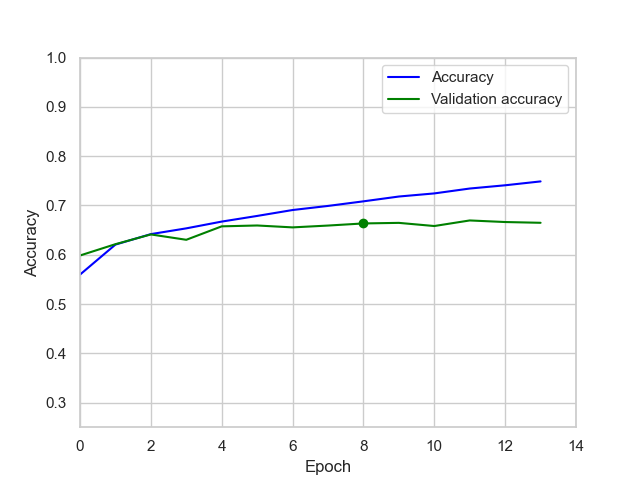
\includegraphics[width=\textwidth]{assets/embedded_classifier_accuracy.png}
    \caption{Accuracy during pretraining of the word embedding model.}
    \label{fig:embedding_model_pretrain}
  \end{subfigure}
  \hfill
  \begin{subfigure}[b]{0.45\textwidth}
    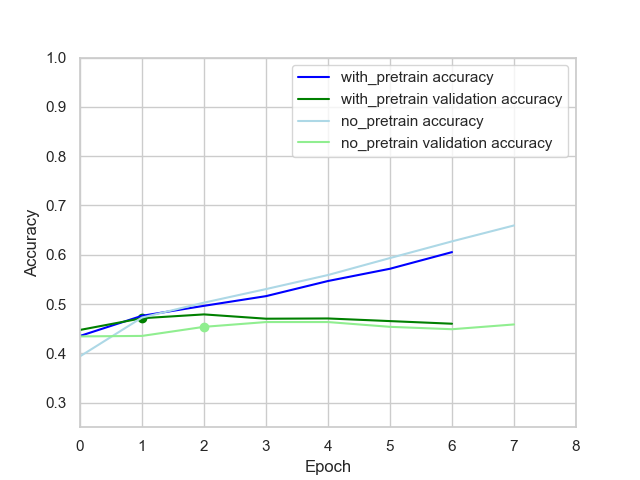
\includegraphics[width=\textwidth]{assets/embedded_classifier_comparison_with_pretrain_no_pretrain.png}
    \caption{Accuracy during training of the word embedding model comparison between model with and without pretraining.}
    \label{fig:embedding_model_train}
  \end{subfigure}
  \caption{Training of the word embedding model.}
  \label{fig:embedding_model_training}
\end{figure}


\vspace*{5ex}
\begin{minipage}{\textwidth}
  \begin{minipage}[b]{0.49\textwidth}
    \centering
      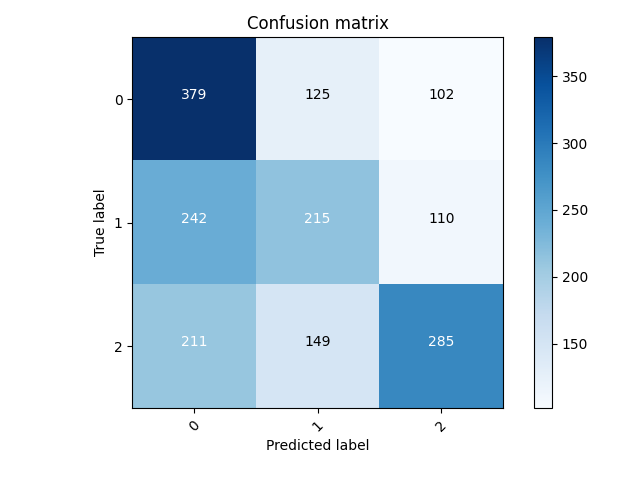
\includegraphics[width=0.8\textwidth]{assets/embedded_model_confusion_matrix.png}
      \captionof{figure}{Confusion matrix on the test set for the pretrained word embedding model.}
      \label{fig:embedding_model_confusion_matrix}
  \end{minipage}
  \hfill
  \begin{minipage}[b]{0.49\textwidth}
    \centering
    \resizebox{0.9\textwidth}{!}{%
    \begin{tabular}[b]{|l|c|c|c|}
      \hline
      \multicolumn{1}{|c|}{label} &precision&recall&f1-score\\ \hline
      0 (entailment)&0.46&0.63&0.53\\
      1 (neutral)&0.44&0.38&0.41\\
      2 (contradiction)&0.57&0.44&0.50\\ \hline
      \multicolumn{3}{|c|}{accuracy} &\multicolumn{1}{c|}{0.48}\\
      \hline
      \end{tabular}}
      \newline
      \captionof{table}{Classification performance on the test set for the pretrained word embedding model.}
      \label{tab:embedding_model_classification_report}
    \end{minipage}
  \end{minipage}


\subsection{Sentence Vector Model (LSTM)}
The sentence vector model was tuned using the keras-tuner, and we tried various combinations of neurons and layers. The results are depicted in Figure~\ref{fig:lstm_hyperparameter_tuning}. Again we trained with the patience set to five, we show the full training graphs where the point marks the epoch with minimal validation loss to which the weights were restored. For the tuning phase, we trained 100,000 samples from the SNLI dataset~\cite{snli-bowman2015}, which we again used for pretraining. 
In the end we choose the architecture depicted in Figure~\ref{fig:lstm_model} with the two non-trainable pre-initialized embedding layers as discussed in Section~\ref{sec:method_lstm}. Followed by two hidden layers for both the premise and the hypothesis with 32 neurons each. Then follows a concatenation and the LSTM layer with 65 units and a dropout of 0.1. After the LSTM there is a hidden layer with 128 neurons followed by the final layer. All Dense layers use the ReLu activation function except for the final layer which as with all other models uses Softmax and has three neurons. Again we train a model with and without pretraining and compare their performance during training in Figure~\ref{fig:lstm_model_train}. For this model, the pretrained version clearly outperformed the version without pretraining. The performance on the test set is listed in Table~\ref{tab:lstm_model_classification_report}. The model reaches a validation accuracy of 0.5 and a test accuracy of 0.5. The f1 score is high for label 0 (entailment) and 2 (contradiction) but low for label 1 (neutral). 

\begin{figure}[h!]
  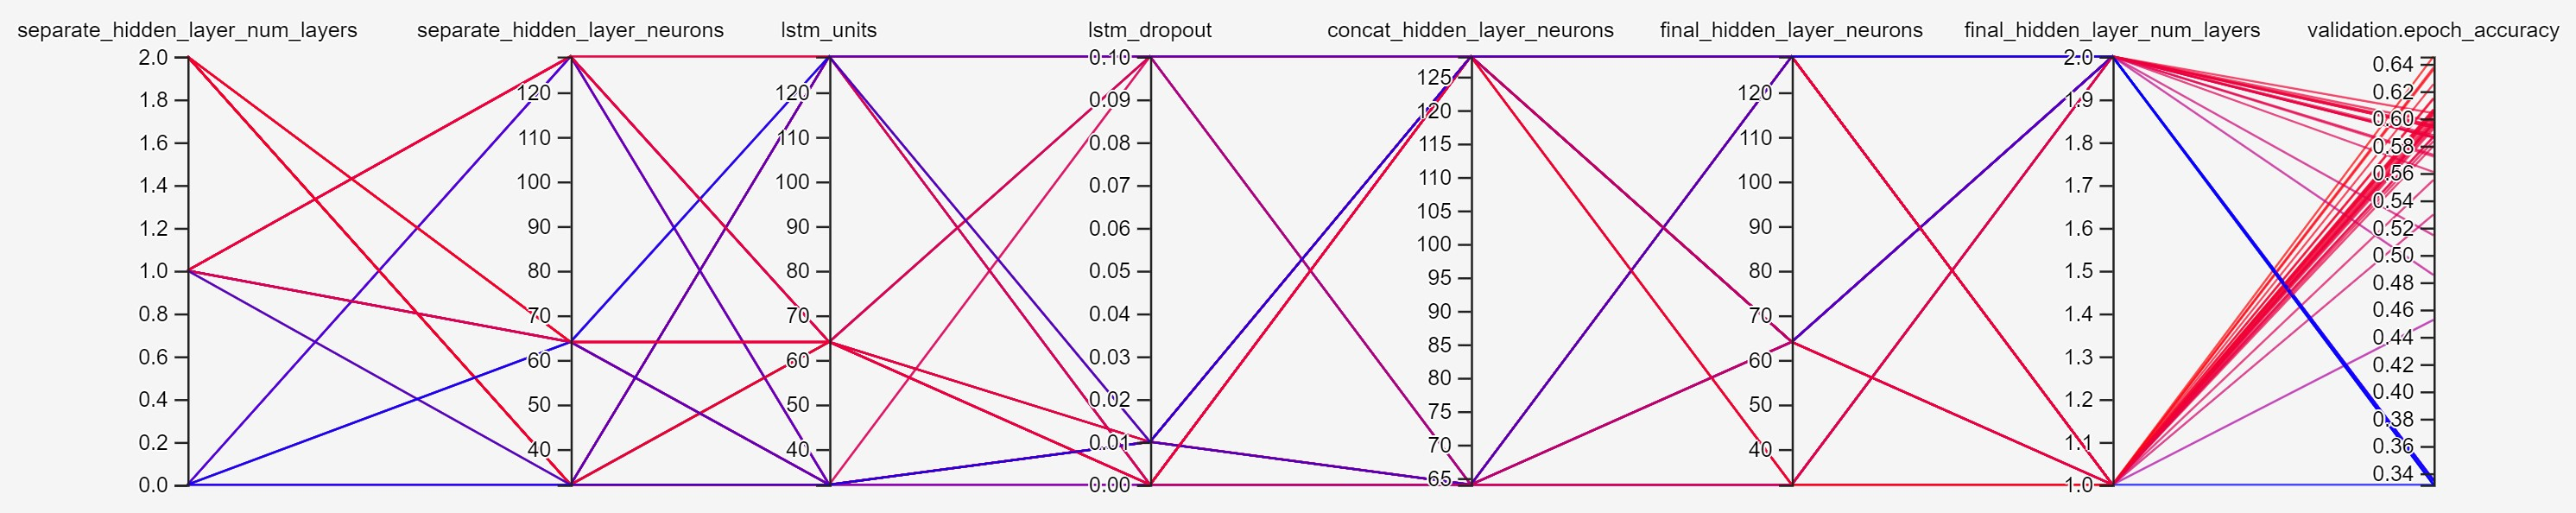
\includegraphics[width=1\textwidth]{assets/lstm_hyper_parameter_tuning.jpg}
  \caption{Sentence vector model hyperparameter tuning using keras-tuner and TensorBoard. The graph is colour-coded by validation accuracy.}
  \label{fig:lstm_hyperparameter_tuning}
\end{figure}

\begin{figure}[!h]
  \begin{subfigure}[b]{0.45\textwidth}
    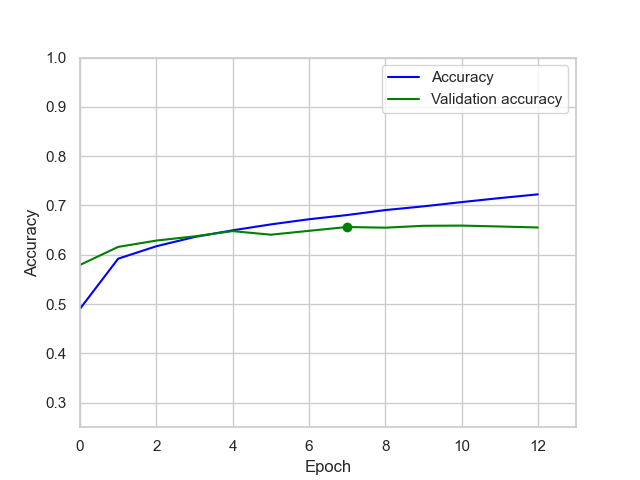
\includegraphics[width=\textwidth]{assets/lstm_classifier_accuracy.png}
    \caption{Accuracy during pretraining of the sentence vector model.}
    \label{fig:lstm_model_pretrain}
  \end{subfigure}
  \hfill
  \begin{subfigure}[b]{0.45\textwidth}
    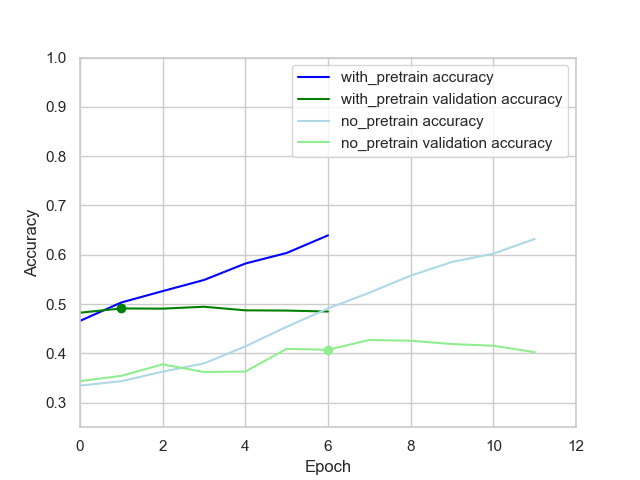
\includegraphics[width=\textwidth]{assets/lstm_classifier_comparison_with_pretrain_no_pretrain.png}
    \caption{Accuracy during training of the sentence vector model comparison between model with and without pretraining.}
    \label{fig:lstm_model_train}
  \end{subfigure}
  \caption{Training of the sentence vector model.}
  \label{fig:lstm_model_training}
\end{figure}


\begin{minipage}[H]{\textwidth}
  \begin{minipage}[b]{0.49\textwidth}
    \centering
    %\rule{6.4cm}{3.6cm}
      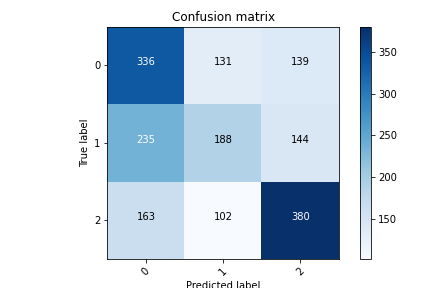
\includegraphics[width=0.8\textwidth]{assets/lstm_model_confusion_matrix.png}
      \captionof{figure}{Confusion matrix on the test set for the LSTM model.}
      \label{fig:lstm_model_confusion_matrix}
  \end{minipage}
  \hfill
  \begin{minipage}[b]{0.49\textwidth}
    \centering
    \resizebox{0.9\textwidth}{!}{%
    \begin{tabular}[b]{|l|c|c|c|}
      \hline
      \multicolumn{1}{|c|}{label}&precision&recall&f1-score\\ \hline
      0 (entailment)&0.46&0.55&0.50\\
      1 (neutral)&0.45&0.33&0.38\\
      2 (contradiction)&0.57&0.59&0.58\\ \hline
      \multicolumn{3}{|c|}{accuracy} &\multicolumn{1}{c|}{0.5}\\
      \hline
      \end{tabular}}
      \newline
      \captionof{table}{Classification performance on the test set for the LSTM model.}
      \label{tab:lstm_model_classification_report}
    \end{minipage}
  \end{minipage}

\subsection{Transformer Models} \label{sec:results_transformer}
We train various different transformers in different sizes and with the two architectures described in Section~\ref{sec:method_transformer} and depicted in Figure~\ref{fig:transformer_models}. However, in our experiments, we did not notice any benefit to the max-pool architecture, as can be seen in Figure~\ref{fig:bert_maxpool_training} where we compare the training performance of both architectures. Therefore we decided to only append a single layer with Softmax activation (Figure~\ref{fig:roberta_model}). Again we pretrain models with 100,000 samples from the SNLI dataset~\cite{snli-bowman2015}. The patience parameter for the transformer models is set to two. We again show the full training graphs and mark the point with minimal validation loss to which the weights were restored. Since the models are already pretrained we expect a small number of training epochs. After training the different models, we compare their validation accuracy and choose the best once for full pretraining in Section~\ref{sec:result_final_transformer_models} where we also show their performance on the test set.

\subsubsection{BERT}
We started with BERT models. We used the \textit{bert-base-cased} as BERT model and the \textit{distilbert-base-cased} model as smaller distilled version also referred to as DistilBERT. Again we train versions with and without pretraining and compare them in Figure~\ref{fig:bert_distilbert_training}. The pretrained version of BERT reached a validation accuracy around 0.6 and clearly outperformed the non-pretrained version. This performance was achieved by pretraining for two epochs and training for one epoch. The smaller DistilBERT version only reached 0.47 with pretraining again outperforming the version without pretraining. DistilBERT was also pretrained for two epochs and trained for one epoch as depicted in Figure~\ref{fig:distilled_bert_model_train} further training did not improve the validation loss and only led to overfitting. 

\begin{figure}[h!]
  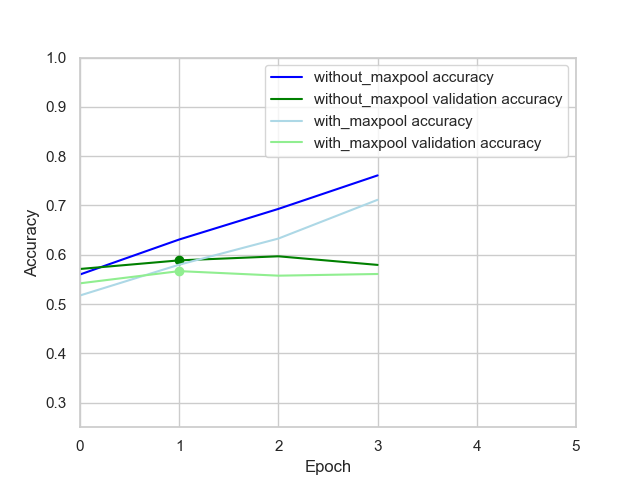
\includegraphics[width=0.4\textwidth]{assets/bert-base-cased_comparison_without_maxpool_with_maxpool.png}
  \caption{Comparison of BERT training with maxpool and with single Softmax layer. Both models are pretrained.}
  \label{fig:bert_maxpool_training}
\end{figure}

\begin{figure}[h!] 
  \begin{subfigure}[b]{0.4\linewidth}
    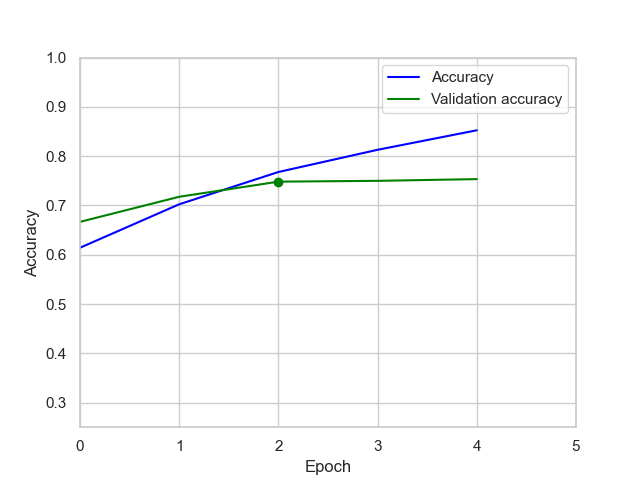
\includegraphics[width=\textwidth]{assets/bert-base-cased_accuracy.png}
    \caption{Accuracy during pretraining of the BERT model.}
    \label{fig:bert_model_pretrain}
    \vspace{2ex}
  \end{subfigure}%% 
  \hfill
  \begin{subfigure}[b]{0.4\linewidth}
    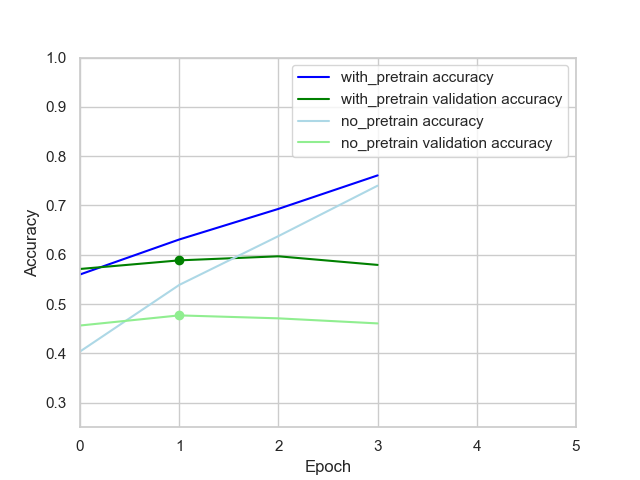
\includegraphics[width=\textwidth]{assets/bert-base-cased_comparison_with_pretrain_no_pretrain.png}
    \caption{Accuracy during training of the BERT model comparison between model with and without pretraining.}
    \label{fig:bert_model_train}
    \vspace{2ex}
  \end{subfigure} 
  \begin{subfigure}[b]{0.4\linewidth}
    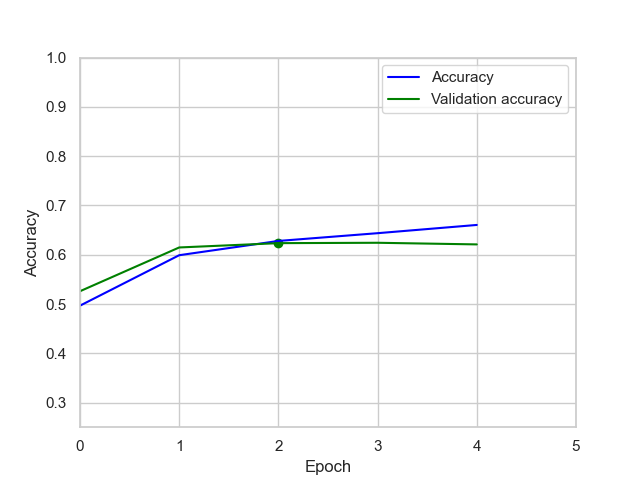
\includegraphics[width=\textwidth]{assets/distilbert-base-cased_accuracy.png}
    \caption{Accuracy during pretraining of the DistilBERT model.}
    \label{fig:distilled_bert_model_pretrain}
  \end{subfigure}%%
  \hfill
  \begin{subfigure}[b]{0.4\linewidth}
    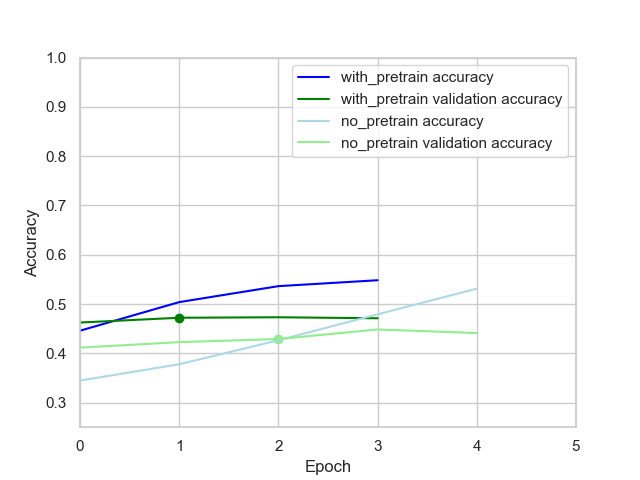
\includegraphics[width=\textwidth]{assets/distilbert-base-cased_comparison_with_pretrain_no_pretrain.png}
    \caption{Accuracy during training of the DistilBERT model comparison between model with and without pretraining.}
    \label{fig:distilled_bert_model_train}
  \end{subfigure} 
  \caption{Training of BERT and DistilBERT models.}
  \label{fig:bert_distilbert_training} 
\end{figure}

\newpage
\subsubsection{RoBERTa}
Next we trained RoBERTa models. We used the standard RoBERTa model \textit{roberta-base} and the smaller \textit{distilroberta-base} as DistilRoBERTa. 
Again we compare the training performance with and without pretraining on 100,000 samples of the SNLI datset~\cite{snli-bowman2015}. The results for the standard RoBERTa model and the distilled version are shown in Figure~\ref{fig:roberta_distilroberta_training}. In both versions, the pretrained version outperformed the non-pretrained version. The larger RoBERTa model with pretraining reached a validation accuracy of 0.8 the distilled version with pretraining reaches 0.74. As shown in Figure~\ref{fig:roberta_model_train} the minimal validation loss is reached after one epoch. %TODO: maybe rewrite and also train on actual data

\begin{figure}[H] 
  \begin{subfigure}[b]{0.4\linewidth}
    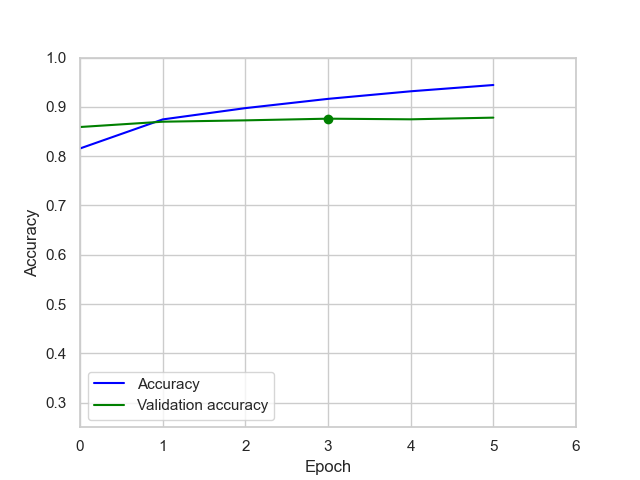
\includegraphics[width=\textwidth]{assets/roberta-base_accuracy.png}
    \caption{Accuracy during pretraining of the RoBERTa model.}
    \label{fig:roberta_model_pretrain}
    \vspace{2ex}
  \end{subfigure}%% 
  \hfill
  \begin{subfigure}[b]{0.4\linewidth}
    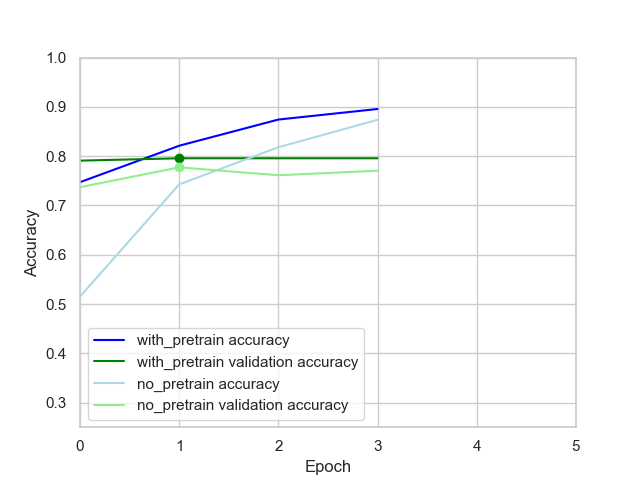
\includegraphics[width=\textwidth]{assets/roberta-base_comparison_with_pretrain_no_pretrain.png}
      \caption{Accuracy during training of the RoBERTa model comparison between model with and without pretraining.}
      \label{fig:roberta_model_train}
    \vspace{2ex}
  \end{subfigure} 
  \begin{subfigure}[b]{0.4\linewidth}
    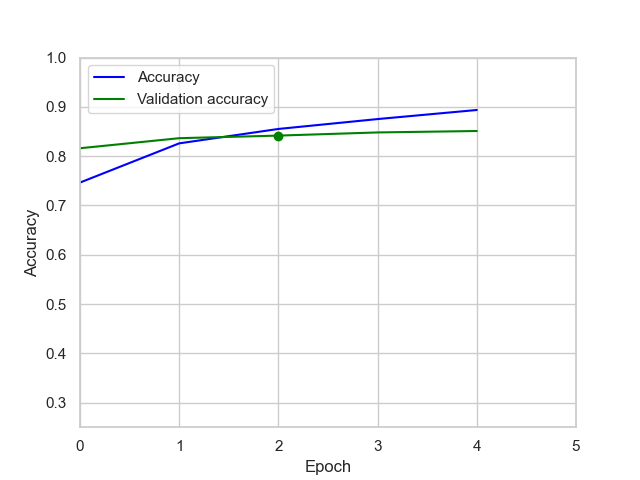
\includegraphics[width=\textwidth]{assets/distilroberta-base_accuracy.png}
    \caption{Accuracy during pretraining of the DistilRoBERTa model.}
    \label{fig:distilled_roberta_model_pretrain}
  \end{subfigure}%%
  \hfill
  \begin{subfigure}[b]{0.4\linewidth}
    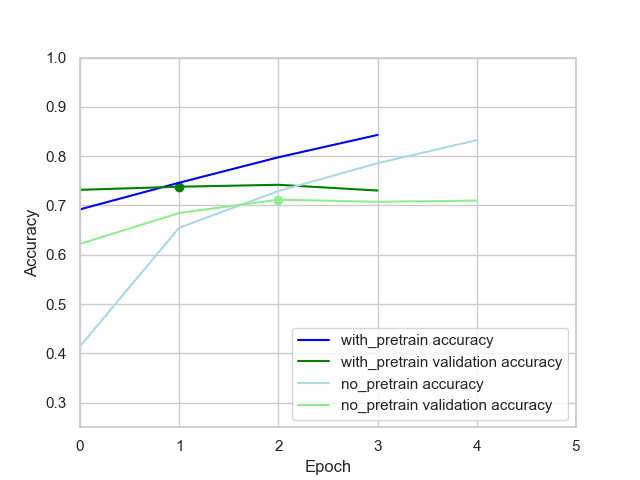
\includegraphics[width=\textwidth]{assets/distilroberta-base_comparison_with_pretrain_no_pretrain.png}
      \caption{Accuracy during training of the DistilRoBERTa model comparison between model with and without pretraining.}
      \label{fig:distilled_roberta_model_train}
  \end{subfigure} 
  \caption{Training of RoBERTa and DistilRoBERTa models.}
  \label{fig:roberta_distilroberta_training} 
\end{figure}

\newpage
\subsubsection{Multilingual Models} \label{sec:multilingual}
Finally, we looked at multilingual models. We trained the multilingual version of BERT \textit{bert-base-multilingual-cased} and the multilingual version of RoBERTa \textit{tf-xlm-roberta-base}. Even though these models can process multiple languages we tried pretraining with the usual 100,000 samples from the english-only SNLI dataset~\cite{snli-bowman2015}. The results are depicted in Figure~\ref{fig:multilang_bert_roberta_training}. The final training for the models was performed on the multilingual data. The pretrained models only outperform the non-pretrained versions by a slight margin. Multilingual BERT with pretraining achieves a validation accuracy of 0.52. Multilingual RoBERTa with pretraining outperforms it's BERT counterpart and achieves 0.72.


\begin{figure}[H] 
  \begin{subfigure}[b]{0.4\linewidth}
    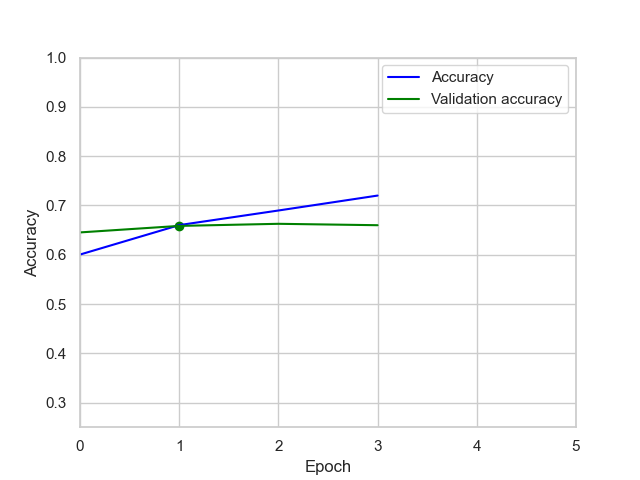
\includegraphics[width=\textwidth]{assets/bert-base-multilingual-cased_accuracy.png}
    \caption{Accuracy during pretraining of the multilingual BERT model.}
    \label{fig:multilingual_bert_model_pretrain}
    \vspace{2ex}
  \end{subfigure}%% 
  \hfill
  \begin{subfigure}[b]{0.4\linewidth}
    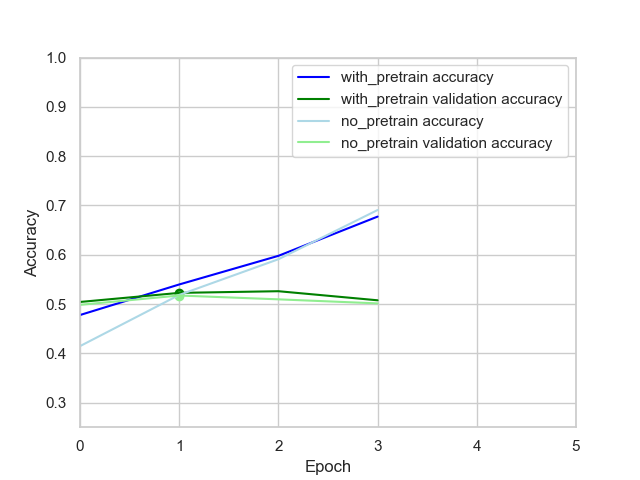
\includegraphics[width=\textwidth]{assets/bert-base-multilingual-cased_comparison_with_pretrain_no_pretrain.png}
    \caption{Accuracy during training of the multilingual BERT model comparison between model with and without pretraining.}
    \label{fig:multilingual_bert_model_train}
    \vspace{2ex}
  \end{subfigure} 
  \begin{subfigure}[b]{0.4\linewidth}
    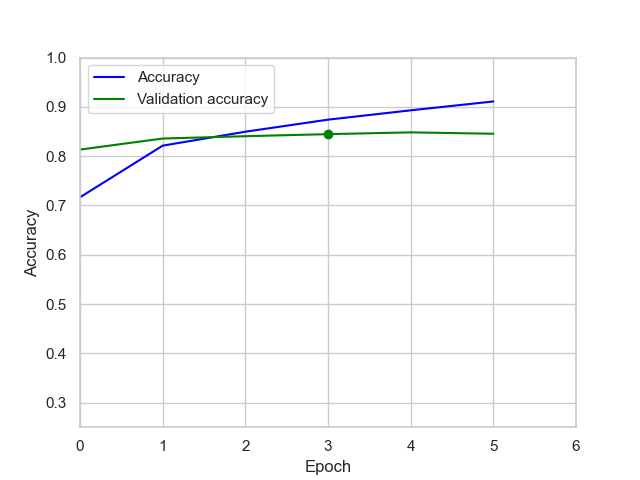
\includegraphics[width=\textwidth]{assets/tf-xlm-roberta-base_accuracy.png}
    \caption{Accuracy during pretraining of the multilingual RoBERTa model.}
    \label{fig:multilingual_roberta_model_pretrain}
  \end{subfigure}%%
  \hfill
  \begin{subfigure}[b]{0.4\linewidth}
    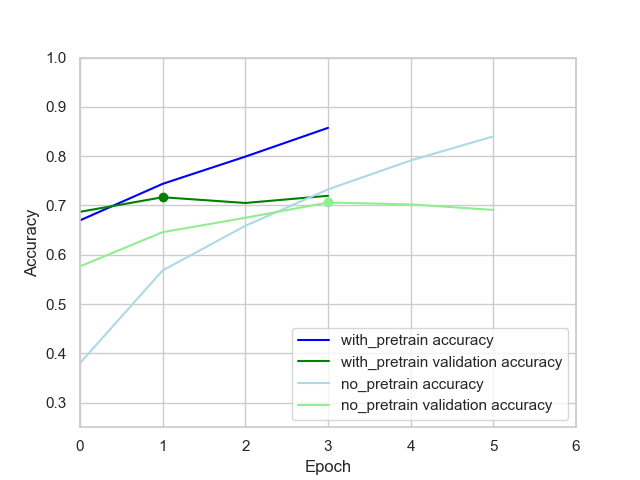
\includegraphics[width=\textwidth]{assets/tf-xlm-roberta-base_comparison_with_pretrain_no_pretrain.png}
    \caption{Accuracy during training of the multilingual RoBERTa model comparison between model with and without pretraining.}
    \label{fig:multilingual_roberta_model_train}
  \end{subfigure} 
  \caption{Training of multilingual versions of BERT and RoBERTa.}
  \label{fig:multilang_bert_roberta_training} 
\end{figure}


\subsection{Final Transformer Models} \label{sec:result_final_transformer_models}
After training different versions of BERT we compared their validation accuracy in Figure~\ref{fig:transformer_comparison}. All RoBERTa models outperformed their BERT counterparts. Furthermore, each model performed better with pretraining. Because of this we choose to further improve the models by pretraining on the entire SNLI datset~\cite{snli-bowman2015} as well as the MultiNLI dataset~\cite{mlni-N18-1101}. This results in a total pretraining data of approximately one million samples. Other than that the training was carried out the same way as described in Section~\ref{sec:results_transformer}. The number of epochs was also similar which is why we omit the training graphs.

\begin{figure}[H]
  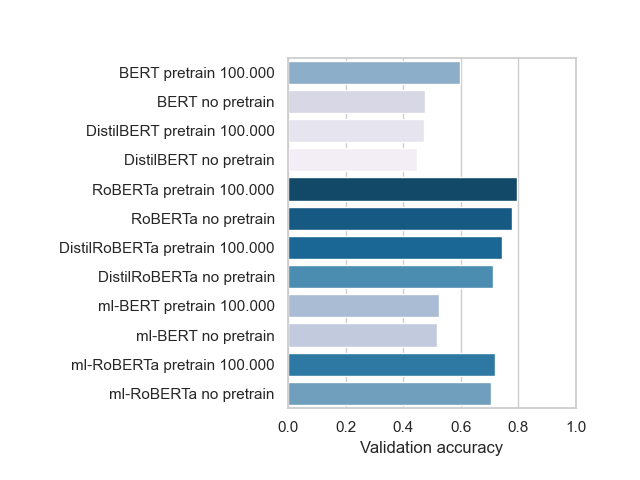
\includegraphics[width=0.7\textwidth]{assets/bert_roberta_comparison.png}
  \caption{Comparison of maximal validation accuracy reached during training for transformer models.}
  \label{fig:transformer_comparison}
\end{figure}


\subsubsection{RoBERTa}
The performance on the held-out test set after pretraining on the combined full pretraining data and training on the Kaggle dataset is listed in Table~\ref{tab:roberta_classification_report}. It achieved a test accuracy of 0.83. The f1-score is particularly high for the contradiction label. The performance difference between the labels can also be observed in the confusion matrix depicted in Figure~\ref{fig:roberta_model_confusion_matrix}.

\vspace*{5ex}
\begin{minipage}[h!]{\textwidth}
  \begin{minipage}[b]{0.49\textwidth}
    \centering
    %\rule{6.4cm}{3.6cm}
      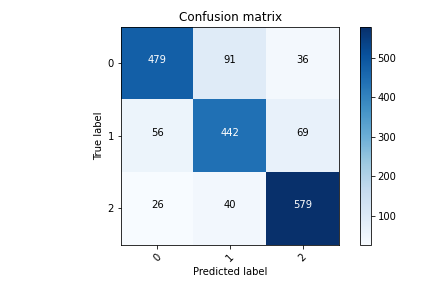
\includegraphics[width=0.8\textwidth]{assets/roberta_confusion_matrix.png}
      \captionof{figure}{Confusion matrix on the test set for the RoBERTa model after full pretraining.}
      \label{fig:roberta_model_confusion_matrix}
  \end{minipage}
  \hfill
  \begin{minipage}[b]{0.49\textwidth}
    \centering
    \resizebox{0.9\textwidth}{!}{%
    \begin{tabular}[b]{|l|c|c|c|}
      \hline
      \multicolumn{1}{|c|}{label}&precision&recall&f1-score\\ \hline
      0 (entailment)&0.85&0.79&0.82\\
      1 (neutral)&0.77&0.78&0.78\\
      2 (contradiction)&0.85&0.90&0.87\\ \hline
      \multicolumn{3}{|c|}{accuracy} &\multicolumn{1}{c|}{0.83}\\
      \hline
      \end{tabular}}
      \newline
      \captionof{table}{Classification performance on the test set for the RoBERTa model after full pretraining.}
      \label{tab:roberta_classification_report}
    \end{minipage}
  \end{minipage}




\subsubsection{DistilRoBERTa}
The performance after full pretraining for the DistilRoBERTa model is listed in Table~\ref{tab:distilroberta_classification_report}. The confusion matrix is plotted in Figure~\ref{fig:distilroberta_model_confusion_matrix}.

\vspace*{5ex}
\begin{minipage}[h!]{\textwidth}
  \begin{minipage}[b]{0.49\textwidth}
    \centering
    %\rule{6.4cm}{3.6cm}
      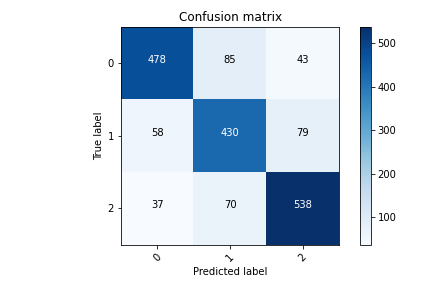
\includegraphics[width=0.8\textwidth]{assets/distilroberta_confusion_matrix.png}
      \captionof{figure}{Confusion matrix on the test set for the DistilRoBERTa model after full pretraining.}
      \label{fig:distilroberta_model_confusion_matrix}
  \end{minipage}
  \hfill
  \begin{minipage}[b]{0.49\textwidth}
    \centering
    \resizebox{0.9\textwidth}{!}{%
    \begin{tabular}[b]{|l|c|c|c|}
      \hline
      \multicolumn{1}{|c|}{label}&precision&recall&f1-score\\ \hline
      0 (entailment)&0.83&0.79&0.81\\
      1 (neutral)&0.74&0.76&0.75\\
      2 (contradiction)&0.82&0.83&0.82\\ \hline
      \multicolumn{3}{|c|}{accuracy} &\multicolumn{1}{c|}{0.80}\\
      \hline
      \end{tabular}}
      \newline
      \captionof{table}{Classification performance on the test set for the DistilRoBERTa model after full pretraining.}
      \label{tab:distilroberta_classification_report}
    \end{minipage}
  \end{minipage}



\subsubsection{Multilingual RoBERTa}
Even though we only have pretraining data available in English, we also use it for pretraining the multilingual model since it improved performance in our initial experiments in Section~\ref{sec:multilingual}. The resulting performance on the test set is listed in Table~\ref{tab:multilingualroberta_classification_report} and the confusion matrix is shown in Figure~\ref{fig:multilingualroberta_model_confusion_matrix}.

\vspace*{5ex}
\begin{minipage}[h!]{\textwidth}
  \begin{minipage}[b]{0.49\textwidth}
      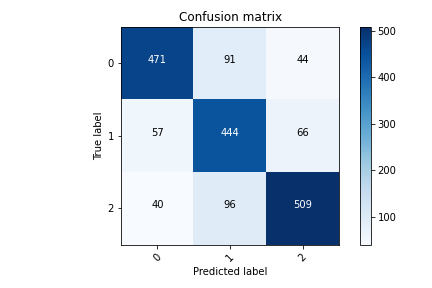
\includegraphics[width=0.9\textwidth]{assets/multilingual_roberta_confusion_matrix.png}
      \captionof{figure}{Confusion matrix on the test set for the Multilingual RoBERTa model after full pretraining.}
      \label{fig:multilingualroberta_model_confusion_matrix}
  \end{minipage}
  \hfill
  \begin{minipage}[b]{0.49\textwidth}
    \centering
    \resizebox{0.9\textwidth}{!}{%
    \begin{tabular}[b]{|l|c|c|c|}
      \hline
      \multicolumn{1}{|c|}{label}&precision&recall&f1-score\\ \hline
      0 (entailment)&0.83&0.78&0.80\\
      1 (neutral)&0.70&0.78&0.74\\
      2 (contradiction)&0.82&0.79&0.81\\ \hline
      \multicolumn{3}{|c|}{accuracy} &\multicolumn{1}{c|}{0.78}\\
      \hline
      \end{tabular}}
      \newline
      \captionof{table}{Classification performance on the test set for the Multilingual RoBERTa model after full pretraining.}
      \label{tab:multilingualroberta_classification_report}
    \end{minipage}
  \end{minipage}


\subsection{Final Model Comparison}
Finally we compare the finished models performance and size in Figure~\ref{fig:test_accuracy_vs_model_size}. Notably the word embedding model is small, because the word embedding vectors are not part of the model. In contrast, the LSTM model contains the embedding vectors, but as non-trainable layers. This is the reason why the LSTM model has a larger model size but the same number of trainable parameters when compared to the word embedding model. We also compare the models trained on the full pretraining data and models only trained on 100,000 samples from SNLI~\cite{snli-bowman2015}. 

\begin{figure}[!h]
  \begin{subfigure}[b]{0.48\textwidth}
    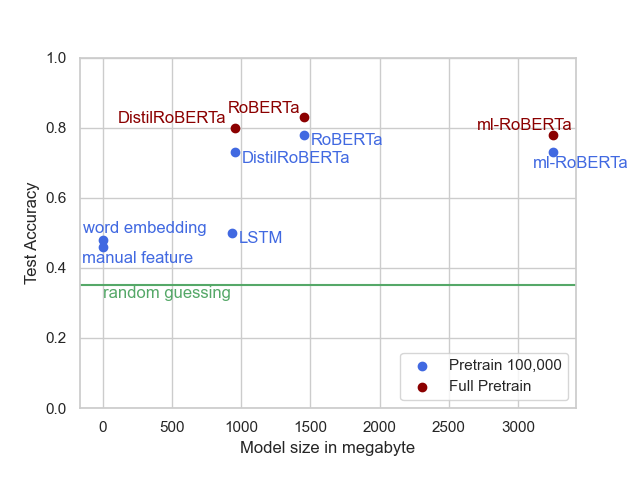
\includegraphics[width=\textwidth]{assets/test_accuracy_vs_model_size.png}
    \caption{Test accuracy compared with model size in Megabyte.}
    \label{fig:test_accuracy_vs_model_size_megabyte}
  \end{subfigure}
  \hfill
  \begin{subfigure}[b]{0.48\textwidth}
    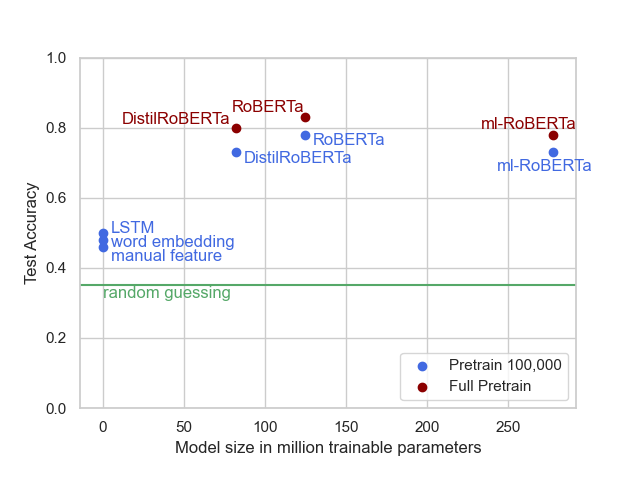
\includegraphics[width=\textwidth]{assets/test_accuracy_vs_trainable_parameters.png}
    \caption{Test accuracy compared with model size in the number of trainable parameters.}
    \label{fig:test_accuracy_vs_model_size_parameters}
  \end{subfigure}
  \caption{Test accuracy of different models compared with their size. Comparison between models trained on the full pretraining dataset and models pretrained on 100,000 samples from SNLI~\cite{snli-bowman2015}.}
  \label{fig:test_accuracy_vs_model_size}
\end{figure}

\subsubsection{English and Multilingual Data}
In Figure~\ref{fig:test_accuracy_english_vs_non_english} we compare the different RoBERTa models trained on the full pretraining dataset. We compare the test accuracy on test data available in English and test data from other languages. 

\begin{figure}[!h]
  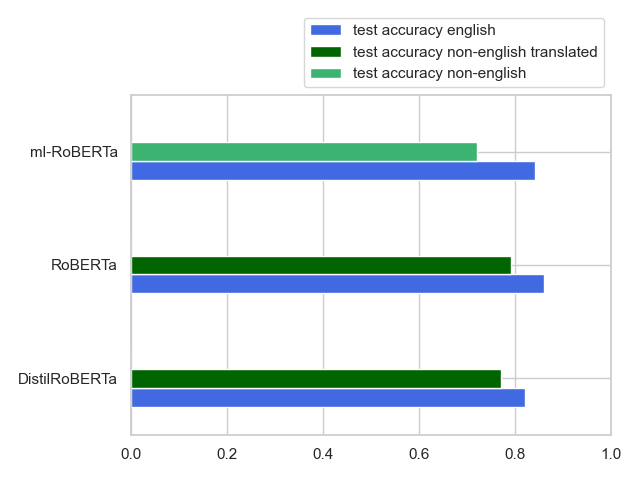
\includegraphics[width=0.5\textwidth]{assets/test_accuracy_english_vs_non_english.png}
  \caption{Comparison of test accuracy of final RoBERTa models on english and non-english samples. While ml-RoBERTa uses the original multilingual data, RoBERTa and DistilRoBERTa use multilingual data translated by Google Translate.}
  \label{fig:test_accuracy_english_vs_non_english}
\end{figure}




\section{Discussion} 
% analyse results and discuss possibilities and limitations of technical approach
\subsection{Pretraining}
For all tested models, pretraining increased the achieved performance. However, the accuracy on the pretraining dataset was always higher than the accuracy of the dataset used for training. This suggests a difference between the pretraining and the training data. In part, this difference can be explained due to part of the training data being translated for the English models. But there might also be other differences between the two datasets.

\subsection{Feature-Based Models}
The more simple feature-based models delivered respectable performance and performed significantly better than the random guessing baseline based on the label distribution. They were able to detect entailment and contradiction specifically well with f1-scores around 0.5 for those labels. In contrast, the f1-score for the label neutral was more close to random guessing. 

\subsection{Sentence Vector Model (LSTM)}
The LSTM model, while performing slightly better when compared to the feature-based models, did not perform as well as we expected. We did not achieve the same accuracy on the SNLI pretraining data as the authors of SNLI~\cite{snli-bowman2015}, which used a similar architecture. However, we do believe this is due to the fact that the embedding vectors we used for our model are significantly smaller. Additionally, we did set them as non-trainable layers. This was done due to the high computational effort required to train the LSTM model. The fact that LSTM models cannot be parallelized to allow for efficient training on GPUs significantly increases the time needed to train them, which is why we had to use this simplified version of the model. 

\subsection{Transformer Models}
When training the transformer models, all RoBERTa models outperformed their BERT counterparts by a significant margin, which is why we only focused on the RoBERTa models for our final evaluation. One type of model missing from our analysis is the large version of BERT, RoBERTa, and their multilingual variant. This was again done due to the computational resources which would be required to train these models. \\
The best model in our testing was RoBERTa with which we achieve similar performance as suggested by the authors of RoBERTa~\cite{roberta-liu2019}. During pretraining we reach 87 percent validation accuracy on the pretraining data. 
The accuracy achieved on the test data of the translated Kaggle dataset~\cite{kaggle-dataset} is lower, however still respectable with 83 percent accuracy. \\
When looking at the comparison of the final models depicted in Figure~\ref{fig:test_accuracy_vs_model_size} we can see that the smaller distilled version of RoBERTa outperforms the significantly bigger multilingual ml-RoBERTa. Of course, the latter does not require translation before using the model. 
However, working with translated data might be a viable option. As Figure~\ref{fig:test_accuracy_english_vs_non_english} illustrates, the performance on translated data, while worse than the performance of data already available in English, is quite good. And the accuracy of the multilingual model on non-English data is significantly worse. One way this could be improved is by pretraining the multilingual model with non-English data. However, finding multilingual datasets is challenging. Another option would be to translate English samples to other languages and use them as pretraining samples. Which we leave as future work.

%TODO: compare with similar work

\section{Conclusion}
% Based on results and analysis what knowledge do you take away from your project?
By using transformer models, we were able to create models that achieve competitive scores for the task of natural language inference on our dataset. We were not able to create an LSTM model that offered comparative performance in part because LSTM models cannot be efficiently trained on GPUs. The distilled version of RoBERTa achieved similar performance to the standard RoBERTa model while being significantly smaller and similar in size to the LSTM model. 
The multilingual version of RoBERTa has the benefit of being able to work with data from different languages. However, the performance was worse compared to the models working with translated data. Therefore depending on the use-case, it might be better to translate non-English data in a pre-processing step and to use an English-only model, for example, in a scenario where multiple classification tasks need to be applied to text data. The input can be translated once and can then be used as input for various English-only models. The alternative would be to create multiple multilingual models, which would need to be significantly bigger in size.  


\pagebreak  

%%
%% The next two lines define the bibliography style to be used, and
%% the bibliography file.
\bibliographystyle{ACM-Reference-Format}
\bibliography{references}


\end{document}
\endinput

